\section{Verification and Validation}
In this section we will run through the initial objectives, and discuss whether each has been achieved.
\subsection{Motors}
\subsubsection{New DC motors}
The new motors have been fully integrated into Tiberius III. They are more efficient, less intrusive, and far more structurally sound than the old ones. As a result of the epicyclic gearboxes and mounting the motors above the wheel axles, Tiberius' ground clearance has been improved by 4cm (see Figure \ref{fig:mech_gc}.
\begin{figure}[!htb]
\begin{center}
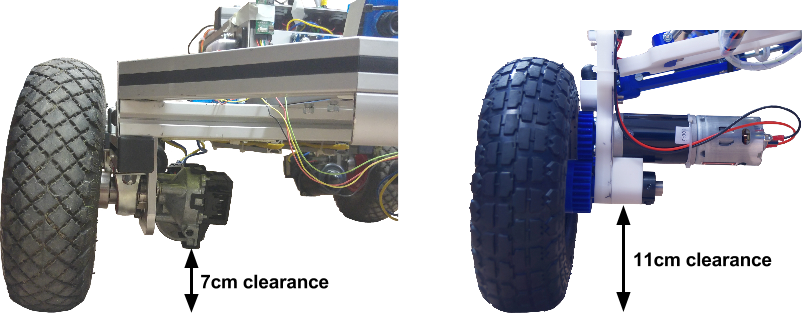
\includegraphics[width=10cm]{mech_ground_clearance_comp.png}
\end{center}
\caption{Comparison between ground clearance of Tiberius II (left) and III (right)}
\label{fig:mech_gc}
\end{figure}
\newline
The motors are also noticeably faster than before - a maximum of 65 RPM, rather than the 42 RPM of the older motors. This has improved Tiberius' maximum speed and turning speed significantly.

\subsubsection{velocity control}
Unfortunately due to time constraints the velocity control objective was not fulfilled. However the hardware infrastructure is in place for controlling the motors by velocity, and the encoder has been tested. The system works in theory, but it will be up to the next group to put it into practice.

\subsubsection{mbed control units}
The mbed boards are in place and working to control the motors. Tiberius III is fully mobile, working from commands from the web interface. While some small aspects of this section are incomplete (e.g. connecting the steering motors as per the above objective) the mbed control units themselves have been installed and are functional.

\subsection{Wheel mounting}
Four modular wheel units have been assembled and are in full working order. Each unit is identical, and includes independent steering and suspension. They are easy to remove and replace, and fulfil this objective fully. While the steering system has not yet been implemented , the steering motors have been tested and are functional.

\subsection{Chassis}
\subsubsection{Reduced chassis}
As stated in Section \ref{Sec:mech_DI_Chassis}, the new chassis uses four metres less aluminium extrusion than before. On top of this, the amount of space for components has been increased dramatically; new 3D printed mounts for components utilising every inch of space mean that the smaller chassis is not giving Tiberius less room for parts.

\subsubsection{Improved wiring standards}
Cable management has been an important aspect of the latter stages of development. Cables are colour coded where possible; red for live wiring, black for ground, with some other colour codes used where appropriate (e.g. purple for raw battery). Colour-coded cable ties have also been used in some areas.
\newline
Part of the cable management system has involved the installation of a wiring board fixed to perspex on one side of the chassis. This board makes it easy to add or remove components to Tiberius' power grid.

\subsubsection{Finalised design iteration}
With the above objectives met it can be agreed that from a mechanical standpoint, Tiberius is nearing completion. Subsequent years' groups can concentrate on the software side of development, in the knowledge that Tiberius' hardware can be left unaltered for the near future. There are still development options (for example, implementation of steering) but this will not involve altering the hardware; all of the necessary infrastructure is already in place.
\begin{figure}[!htb]
\begin{center}
\includegraphics[width=12cm]{mech_Tib3.png}
\end{center}
\caption{Tiberius III}
\label{fig:mech_tib3}
\end{figure}